\documentclass[12pt]{article}

\usepackage{graphicx}
\usepackage{paralist}
\usepackage{listings}
\usepackage{booktabs}
\usepackage{hyperref}

\oddsidemargin 0mm
\evensidemargin 0mm
\textwidth 160mm
\textheight 200mm

\pagestyle {plain}
\pagenumbering{arabic}

\newcounter{stepnum}

\title{CS/SE 2XB3 Lab 2 Report}
\author{
  Wang, Mingzhe\\
  \texttt{wangm235@mcmaster.ca}
  \and
  Li, Xing\\
  \texttt{li64@mcmaster.ca}
  \and
  Moon, Hyosik\\
  \texttt{moonh8@mcmaster.ca}
  }
\date{\today}

\begin{document}

\maketitle

This report concludes the main observations that we found in this week's lab, with the analysis that we did for the experiments of each methods.

\section{Timing Data}
In this part, we will analyze the test results of three functions and give our best determination of how each of these functions is growing in $n$.
\subsection{Timing \(f(n)\) data}
For the data set of \(f(n)\), the trend line looks like linear. From the chart below we can see that the \(R^2\) is 0.9992 for the linear equation. It is already a very good result.

\begin{figure}[h!]
\centering
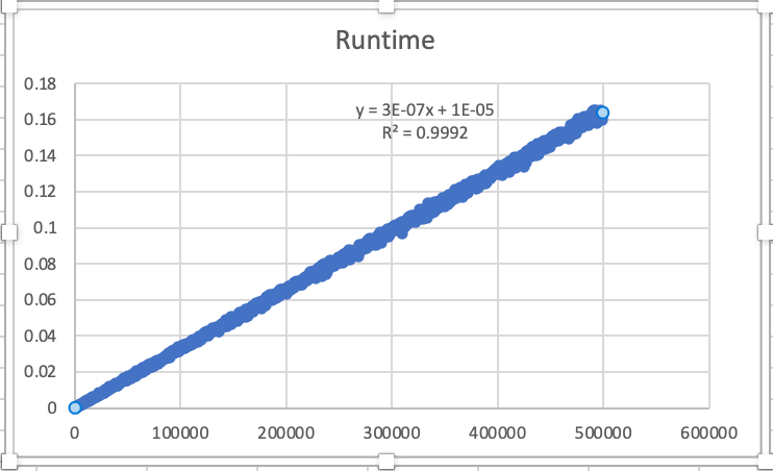
\includegraphics[width=0.6\textwidth,height=\textheight,keepaspectratio]{fn_1.png}
\caption{linear fitting for $f(n)$}
\label{Figure: fn_1}
\end{figure}

\newpage Therefore, we can conclude that $f(n) \sim O(n)$.

\subsection{Timing \(g(n)\) data}
For the data set of \(g(n)\), the trend line looks not linear. From the chart below we can see that the $R^2$ is only 0.7974 for the linear model.

\begin{figure}[h!]
\centering
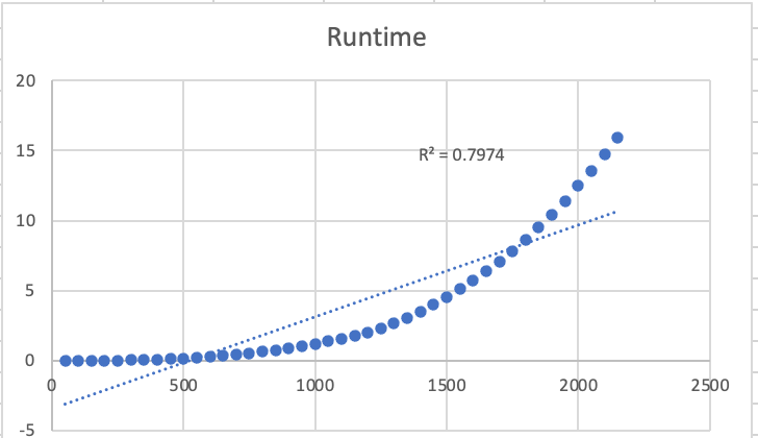
\includegraphics[width=0.6\textwidth,height=\textheight,keepaspectratio]{gn_1.png}
\caption{linear fitting for $g(n)$}
\label{Figure: gn_1}
\end{figure}

~\newline\noindent With Polynomial model, $R^2$ is 0.9883 for quadratic and 0.9999 for cubic. 
\begin{figure}[h!]
\centering
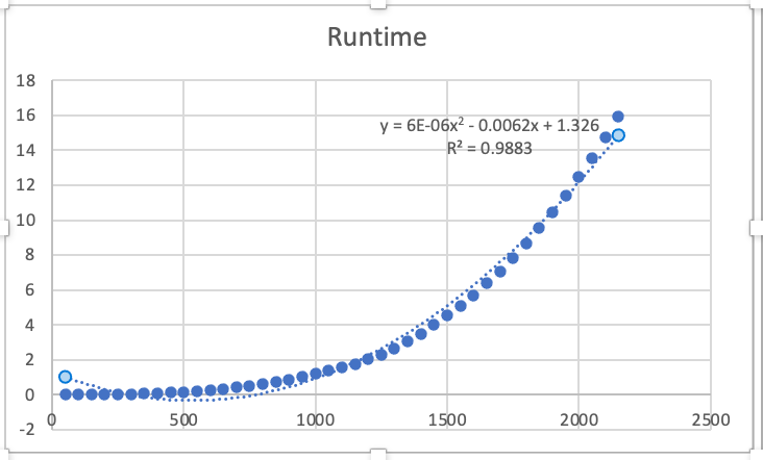
\includegraphics[width=0.6\textwidth,height=\textheight,keepaspectratio]{gn_2.png}
\caption{quadratic fitting for $g(n)$}
\label{Figure: gn_2}
\end{figure}

\begin{figure}[h!]
\centering
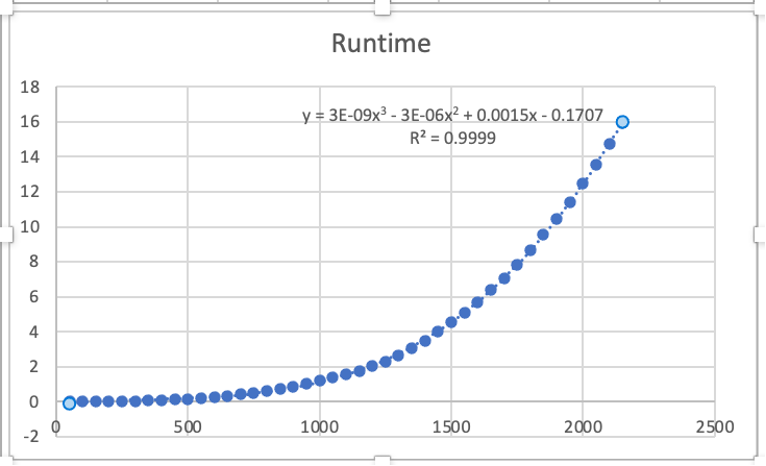
\includegraphics[width=0.6\textwidth,height=\textheight,keepaspectratio]{gn_3.png}
\caption{cubic fitting for $g(n)$}
\label{Figure: gn_3}
\end{figure}

\newpage ~\newline\noindent Therefore, we can conclude $g(n) \sim O(n^3)$

\subsection{Timing \(h(n)\) data}
For the data set of $h(n)$, the trend line looks like linear, but it starts to deviate when the $n$ is greater than 400,000. 

\begin{figure}[h!]
\centering
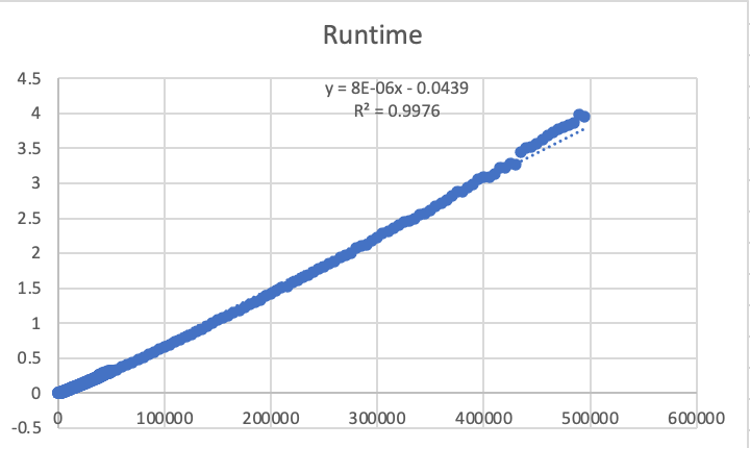
\includegraphics[width=0.6\textwidth,height=\textheight,keepaspectratio]{hn_1.png}
\caption{linear fitting for \(h(n)\)}
\label{Figure: hn_1}
\end{figure}

\newpage ~\newline\noindent Is it possible that it is actually $O(nlogn)$? We created a new series by dividing the runtime $h(n)$ by $n$, multiplying by 500,000, and fitting in a logarithmic model. The $R^2$ is 0.9612. If $h(n) \sim O(n)$, $h(n)/n$ should be a constant; if $h(n) \sim O(nlogn)$, $h(n)/n$ should be logarithmic. It seems $O(nlogn)$ is better to describe $h(n)$.

\begin{figure}[h!]
\centering
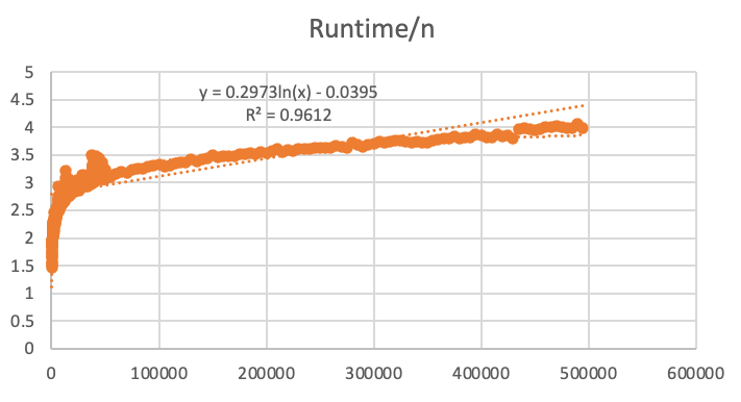
\includegraphics[width=0.6\textwidth,height=\textheight,keepaspectratio]{hn_2.png}
\label{Figure: hn_2}
\caption{logarithmic fitting for \(h(n)/n\)}
\end{figure}

~\newline\noindent Therefore, we conclude that the best estimate with the given data is $h(n) \sim O(nlogn)$.



\section{Python Lists}
In this part, we will analyze the performance of three Python list methods, and give our conclusion about their time complexity and the corresponding reasoning.
\subsection{Copy}
\begin{enumerate}[(1)]
\item \textbf{Description of test method}\\
To test the \verb|copy()| method, first we define a \verb|create_random_list(n, upper)| method that creates a list of length \verb|n| with random integers in the range of \verb|[0, upper)| as elements. For each test, i.e. each possible value of \verb|n|, there are runs with the number of \verb|runs|. This design is to exclude possible distraction to show a more concise trending. For each run, a list \verb|ls| is created first, then the time counter starts to record the actual running time of  \verb|ls.copy|. When all runs for each possible \verb|n| value are finished, the average running time of \verb|ls.copy| will be returned. \\\\
We also implement \verb|plot_copy_test| to plot or get the data of the test result, the work principle of the methods are returning a \verb|y| representing the y-coordinates by a given \verb|x| representing the x-coordinates to plot the scatter diagram or return the data set. It should be noted that we use the \verb|xlsxwriter| package to automatically write the data to excel files.\\\\
The source code for this part is as the following:
\lstset{language=Python, basicstyle=\ttfamily\small, breaklines=true, showspaces=false,
  showstringspaces=false, breakatwhitespace=true}
\begin{lstlisting}
import matplotlib.pyplot as plt
import random
import timeit
import xlsxwriter

data_path = r'/Users/kidsama/Documents/COMPSCI 2XB3/2xb3_lab2/list_data.xlsx'
workbook = xlsxwriter.Workbook(data_path)

def create_random_list(n, upper):
    return [random.randint(0, upper) for _ in range(n)]

# def copy test
def copy_test(runs, n, upper):
    total = 0
    for _ in range(runs):
        ls = create_random_list(n, upper)
        start = timeit.default_timer()
        ls.copy()
        end = timeit.default_timer()
        total += end - start
    return total/runs

# plot copy test
def plot_copy_test():
    x = [_ * 100 for _ in range(100)]
    y = []
    for _ in x:
        y.append(copy_test(100, _, 500))
    plt.scatter(x, y, marker='.')
    plt.xlabel('N ')
    plt.ylabel('T (s)')
    plt.title('Time complexity of copy())')
    copy_test_data = workbook.add_worksheet("copy_test_data")
    copy_test_data.write(0, 0, "N")
    copy_test_data.write_column(1, 0, x)
    copy_test_data.write(0, 1, "T")
    copy_test_data.write_column(1, 1, y)
\end{lstlisting}

\item \textbf{Observations and conclusion}\\
From the scatter diagram derived from the test data, we conclude that the time complexity of \verb|copy()| is \(O(n)\), where \(n\) is the input size \--- the length of the argument list.

\begin{figure}[h!]
\centering
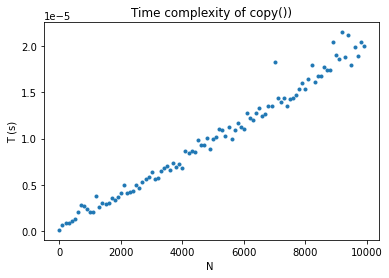
\includegraphics[width=0.6\textwidth,height=\textheight,keepaspectratio]{figure_1.png}
\caption{scatter plot of copy() test}
\label{Figure: 1}
\end{figure}

\newpage \item \textbf{Evidence}\\
We back up our observation by plotting the trend line of this scatter diagram and determine which one is best fitted using \(R^2\).

\begin{figure}[h!]
\centering
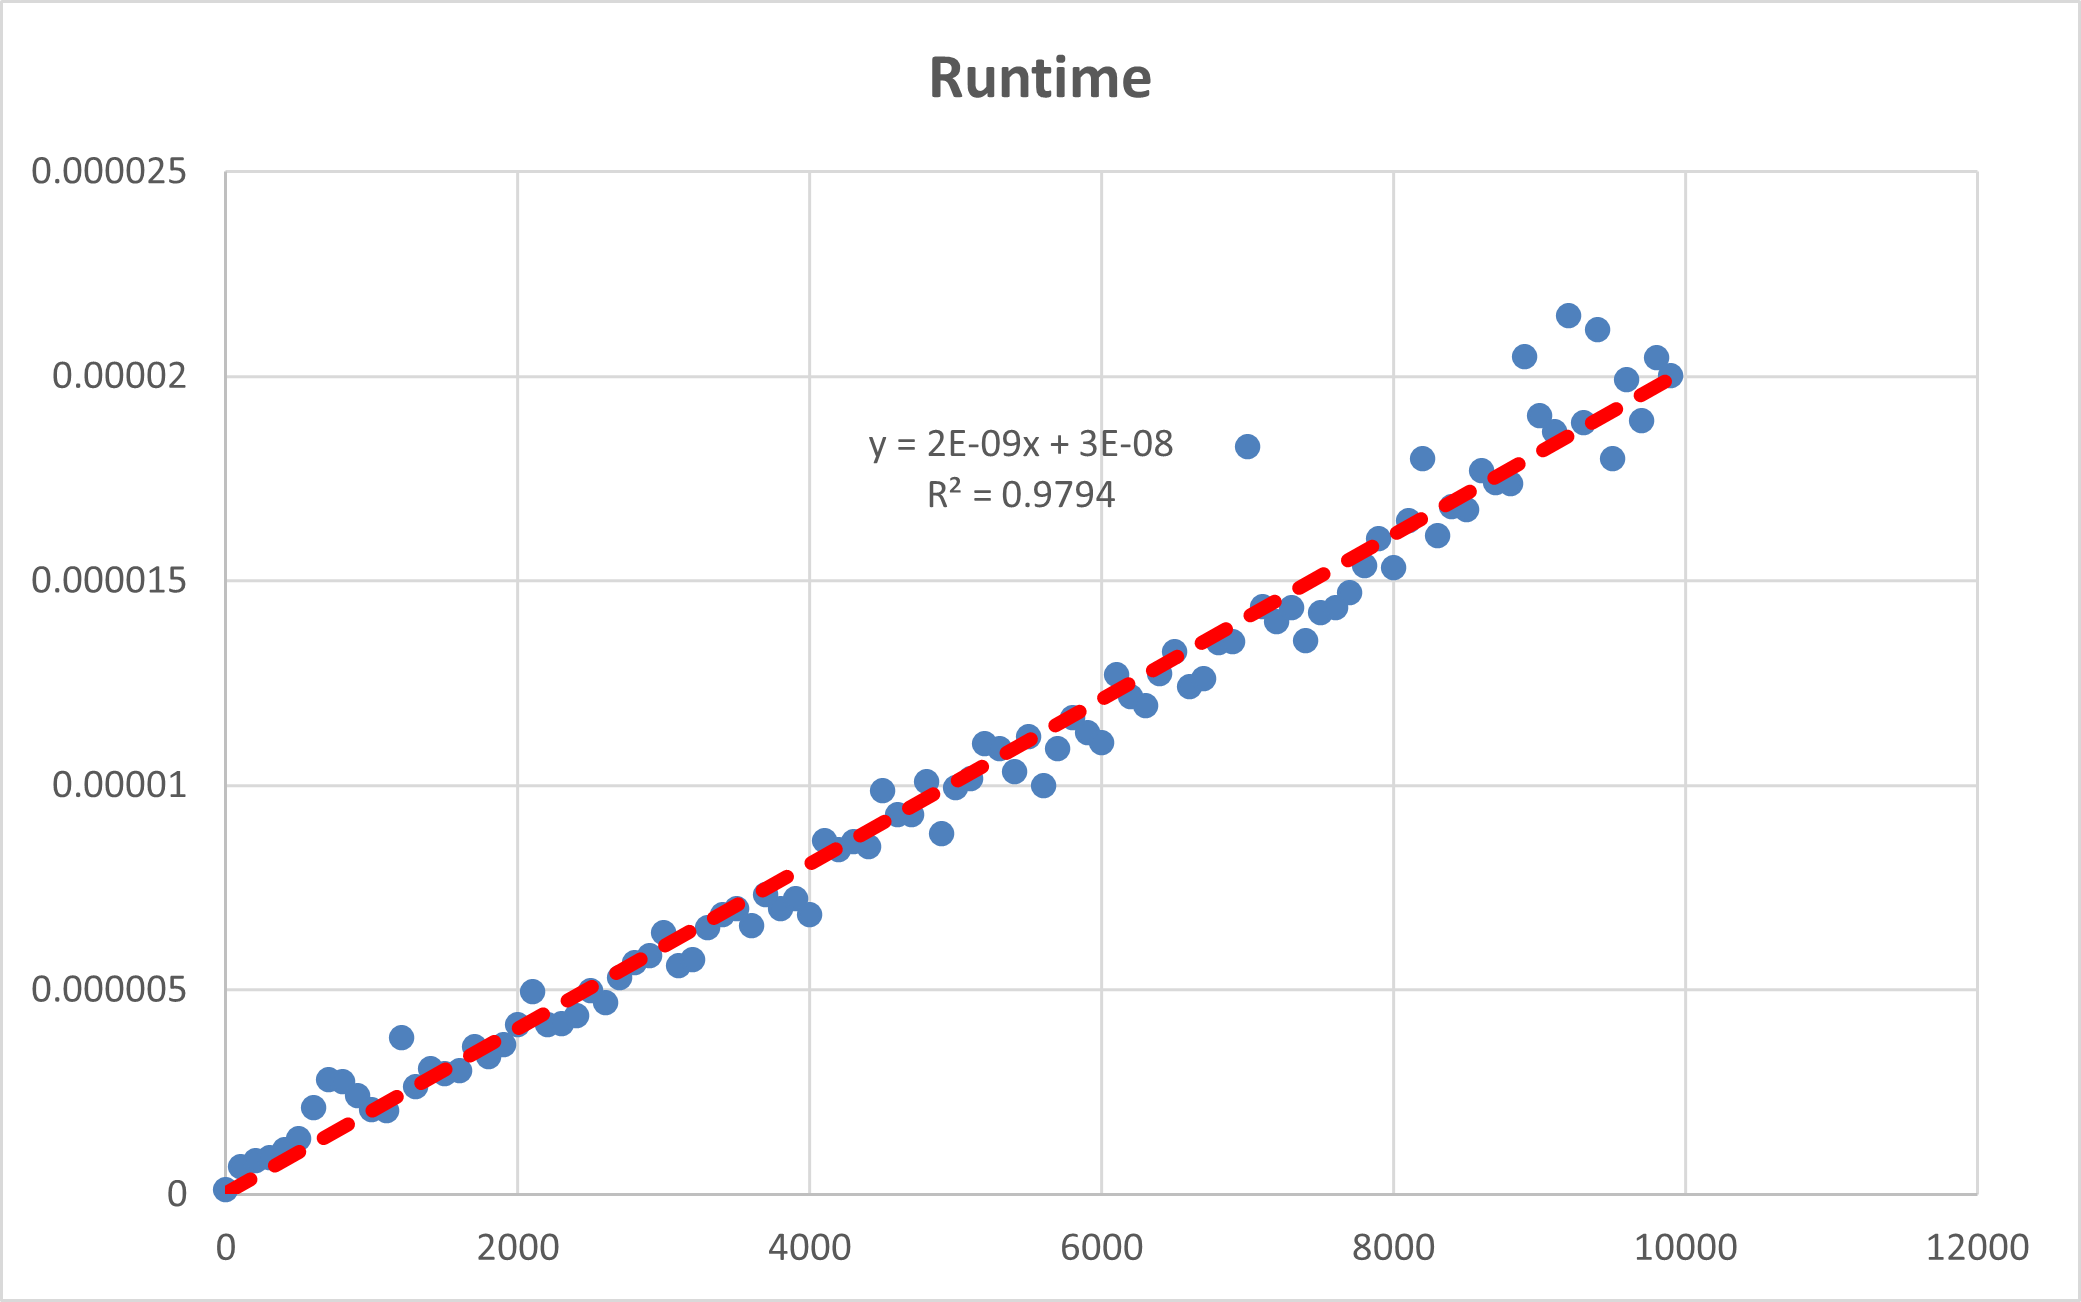
\includegraphics[width=0.6\textwidth,height=\textheight,keepaspectratio]{picture/copy.png}
\caption{linear fitting for copy() test}
\label{copy}
\end{figure}

Apparently, for linear trending line, \(R^2\) is equal 0.9794, which is enough for us to verify the conclusion.

\item \textbf{Explanation}\\
Through the research, we find that \verb|copy()| in Python is actually a shallow copy. A shallow copy creates a new list object, but it does not create new list elements. Instead, it simply copies the references to these objects. In other word, Python goes over all elements in the list and adds a copy of the object reference to the new list (copy by reference). Thus, the time complexity of \verb|copy()| is \(O(n)\).
\begin{figure}[h!]
\centering
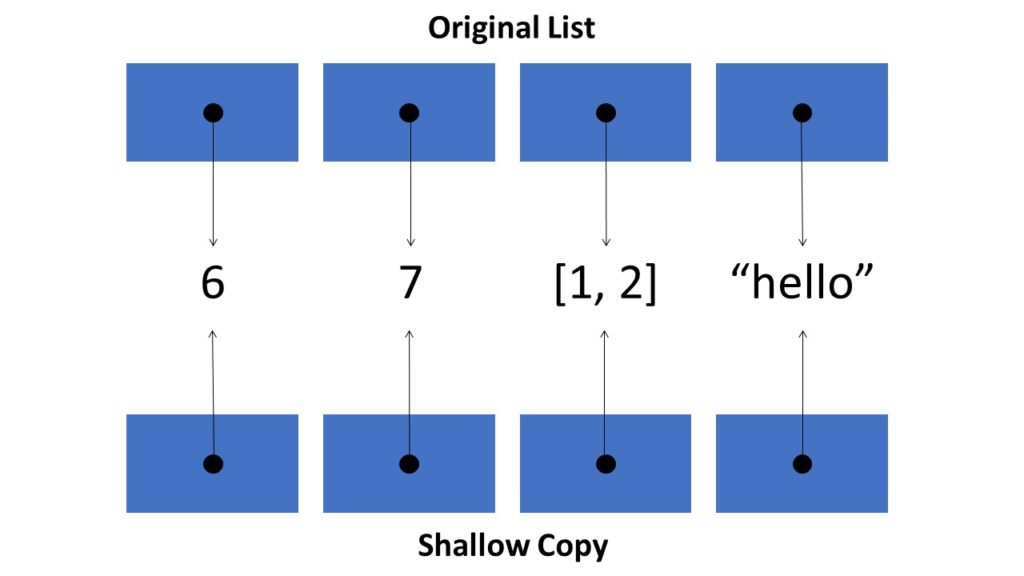
\includegraphics[width=0.6\textwidth,height=0.3\textheight,keepaspectratio]{shallow_copy.jpg}
\caption{example of Python shallow copy}
\label{shallow_copy}
\end{figure}


\end{enumerate}
\subsection{Lookups}
\begin{enumerate}[(1)]
\item \textbf{Predictions}\\
Before we starting the test, our prediction is that the time complexity of \verb|lookups|, i.e. \verb|L[i]| is  \(O(n)\), where n is the max index of the item we looking for. Because in our theory courses, we are taught that the time complexity of traversing a linked list of length \verb|n| to find a value is \(O(n)\) in the worst case.
\item \textbf{The original scatter plot}\\
To follow the professor's instructions strictly, we reduce the abstractions, i.e. the number of subroutines, in our implementation. That means all the statements are written in a single function. Our first version of test function \verb|plot_lookups_test| is as the following:

\lstset{language=Python, basicstyle=\ttfamily\small, breaklines=true, showspaces=false,
  showstringspaces=false, breakatwhitespace=true}
\begin{lstlisting}
def plot_lookups_test():
    ls = create_random_list(1000000, 1000000)
    x = range(1000000)
    y = []
    for i in x:
        start = timeit.default_timer()
        ls[i]
        end = timeit.default_timer()
        y.append(end - start)
    plt.scatter(x, y, marker='.')
\end{lstlisting}

It provides the first version of the scatter plot.

\begin{figure}[h!]
\centering
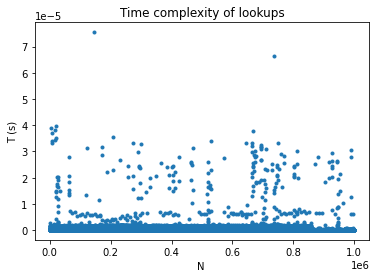
\includegraphics[width=0.6\textwidth,height=\textheight,keepaspectratio]{figure_2.png}
\caption{original scatter plot for lookups}
\label{Figure: 2}
\end{figure}

\item \textbf{Potential problems and corresponding fix}\\
Although the scatter plot shows certain trending of the complexity, there are some issues \--- there are too many outliers in the plot, which could reduce the goodness of fit in our next steps. To fix this issue, we apply a similar strategy as used in the \verb|Copy()| test. For each possible value of \verb|n|, we will run 500 times same tests and calculate the average time, which we expect can reduce the noises from irrelevant factors, like the OS, the concurrent programs, etc. The fixed version of test function \verb|plot_lookups_test| is as the following:
\lstset{language=Python, basicstyle=\ttfamily\small, breaklines=true, showspaces=false,
  showstringspaces=false, breakatwhitespace=true}
\begin{lstlisting}
def plot_lookups_test_fixed(runs):
    ls = create_random_list(1000000, 1000000)
    x = range(1000000)
    y = []
    for i in x:
        for _ in range(runs):
            total = 0
            start = timeit.default_timer()
            ls[i]
            end = timeit.default_timer()
            total += end - start
        y.append(total/runs)
    plt.scatter(x, y, marker='.')
    plt.xlabel('N ')
    plt.ylabel('T (s)')
    plt.title('Time complexity of lookups')
    copy_test_data = workbook.add_worksheet("lookups_test_data")
    copy_test_data.write(0, 0, "N")
    copy_test_data.write_column(1, 0, x)
    copy_test_data.write(0, 1, "T")
    copy_test_data.write_column(1, 1, y)
\end{lstlisting}
\item \textbf{The revised scatter plot}\\
After fixing that issue, we rerun the experiment. As showed in Figure \ref{Figure: 3}, the number of outliers in the scatter diagram is smaller.

\begin{figure}[h!]
\centering
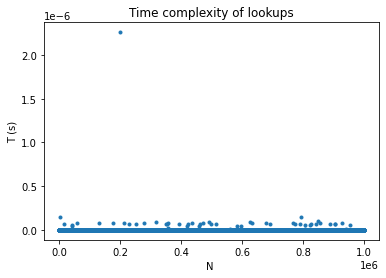
\includegraphics[width=0.6\textwidth,height=\textheight,keepaspectratio]{figure_3.png}
\caption{revised scatter plot for lookups}
\label{Figure: 3}
\end{figure}

Then we export our data to excel to draw the trending line. Among all possible fitting functions, the constant line is the best.

\begin{figure}[h!]
\centering
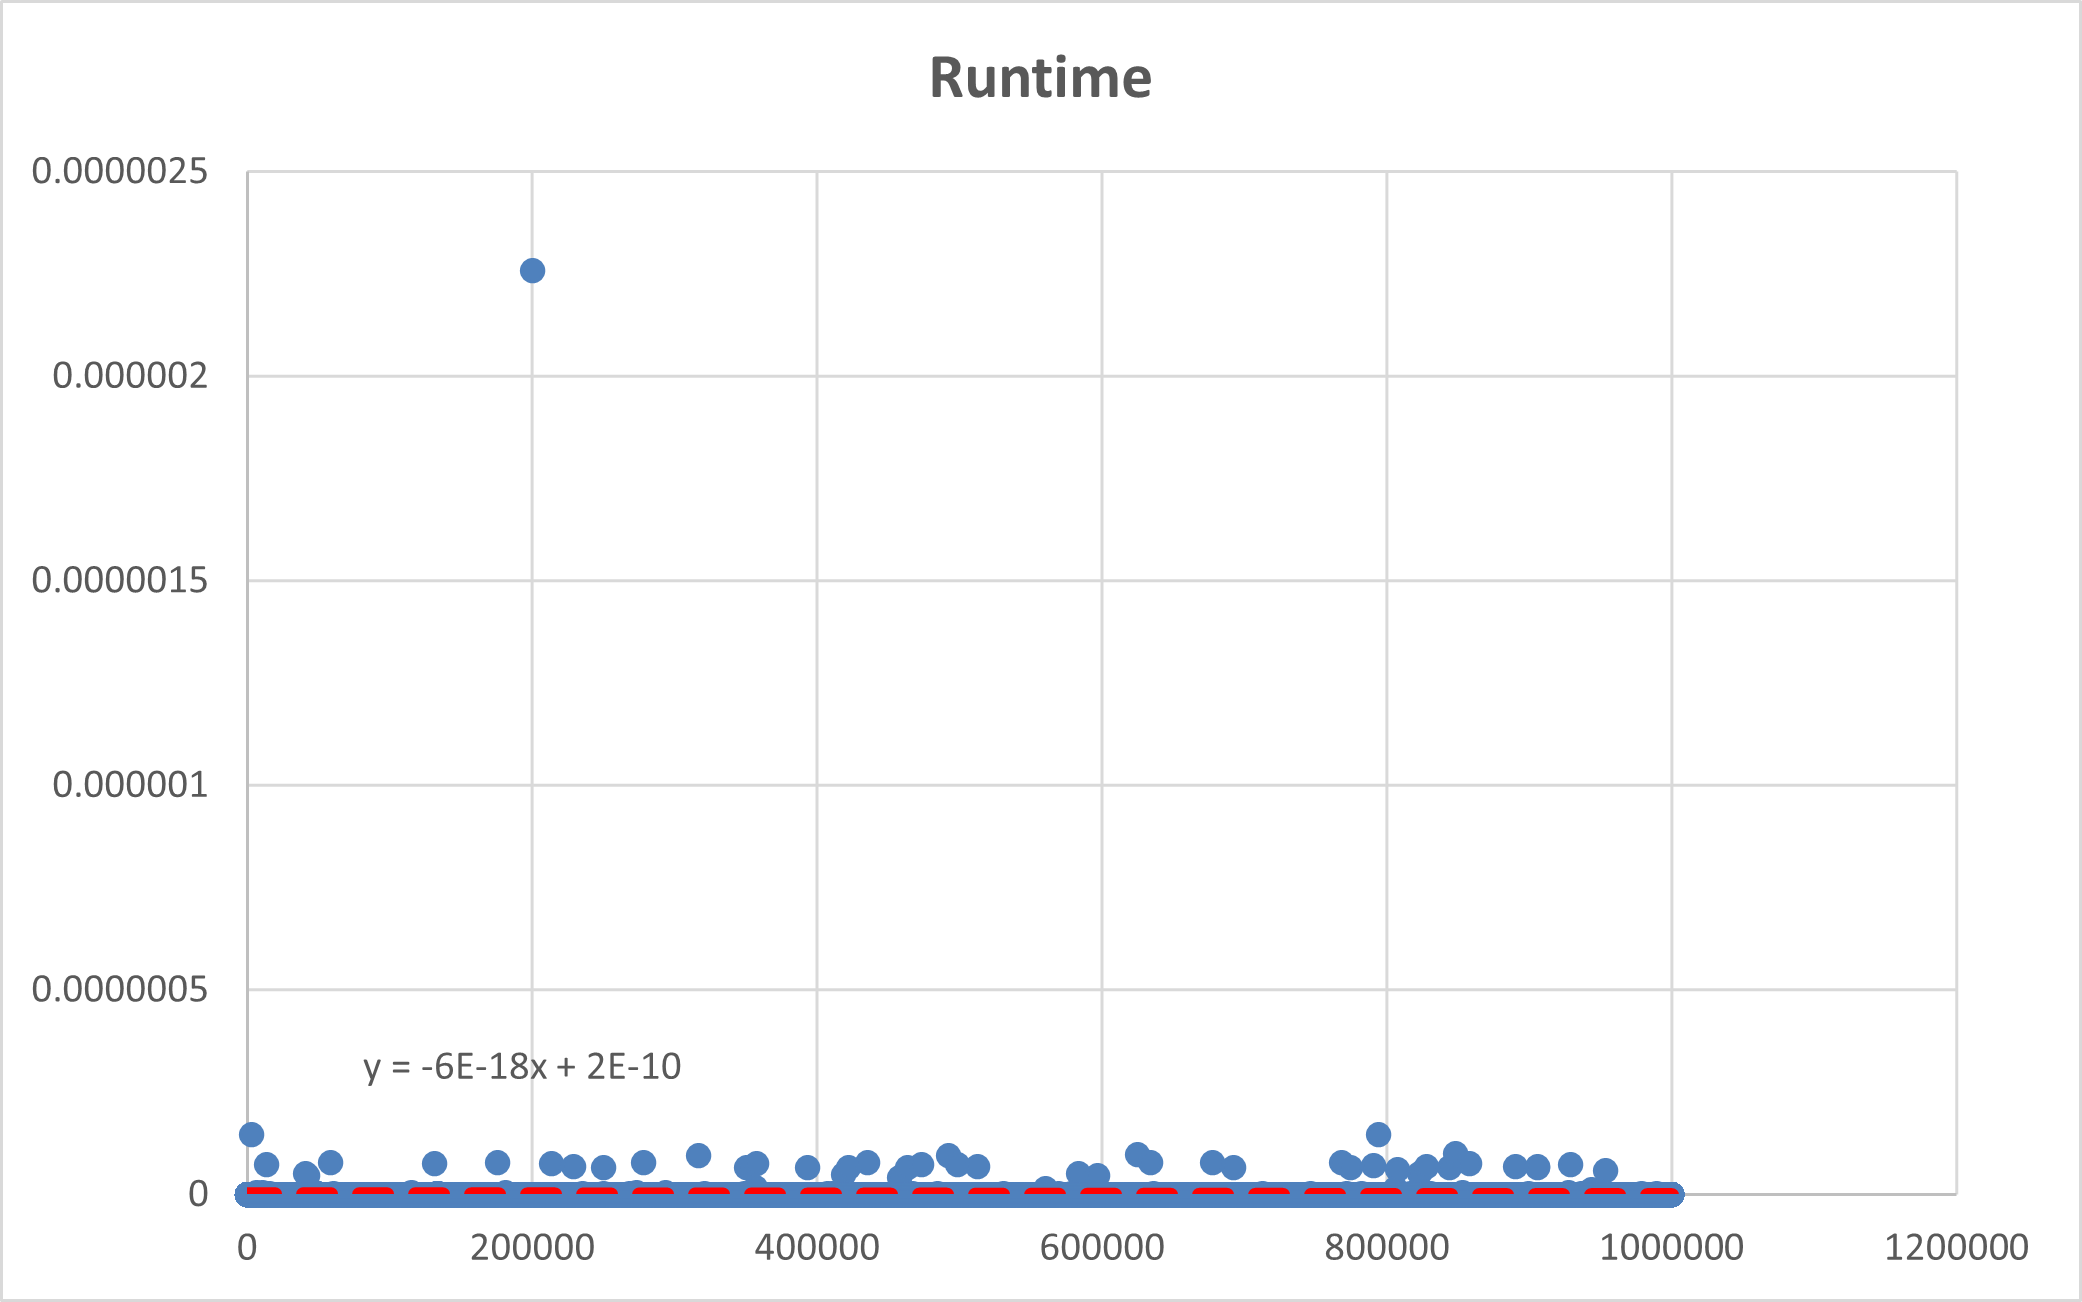
\includegraphics[width=0.6\textwidth,height=\textheight,keepaspectratio]{picture/lookups.png}
\caption{constant fitting for lookups}
\label{Figure: 4}
\end{figure}

\newpage \item \textbf{Conclusion}\\
The observation of our tests does not support our prediction that the run time of \verb|lookups|, i.e. \verb|L[i]| is  \(O(n)\) in the worst case. Instead, it shows that whatever the \(i\) is, the corresponding runtime is always a constant. \\\\
Our explanation is that the \verb|list| type of Python is actually an array rather than a linked list. Thus, we can randomly access the data in the Python lists using their indexes in a constant time, which means the time complexity of this process is \(O(n)\).
\end{enumerate}
\subsection{Append}
\begin{enumerate}[(1)]
\item \textbf{Prediction}\\
Before we starting the test, again we create our prediction \-- the time complexity of \verb|append()|, i.e. \verb|list1.append(a)| is \(O(1)\). The reason is that \verb|append()| is a mutator that will mutate the current object. That means to achieve the `append' behavior, it simply add a reference of the argument to the end of the array, which takes a constant time.
\item \textbf{The implementation}\\
Following the design principle of lookups tests, we design our test function as the following:
\lstset{language=Python, basicstyle=\ttfamily\small, breaklines=true, showspaces=false,
  showstringspaces=false, breakatwhitespace=true}
\begin{lstlisting}
def plot_append_test_fixed(runs):
    x = range(1000000)
    y = []
    ls = []
    for i in x:
        for _ in range(runs):
            total = 0
            value = random.randint(0, 1000000)
            start = timeit.default_timer()
            ls.append(value)
            end = timeit.default_timer()
            total += end - start
        y.append(total/runs)
    plt.scatter(x, y, marker='.')
    plt.xlabel('N ')
    plt.ylabel('T (s)')
    plt.title('Time complexity of append()')
    copy_test_data = workbook.add_worksheet("append_test_data1")
    copy_test_data.write(0, 0, "N")
    copy_test_data.write_column(1, 0, x)
    copy_test_data.write(0, 1, "T")
    copy_test_data.write_column(1, 1, y)
\end{lstlisting}
The run times of the same tests for each possible value of \verb|x| is set to be 100. As mentioned in the instruction, we instantiate the current list with one million random integers in the range of \([0, 1000000)\).

\item \textbf{Scatter plot and trend line}\\
This time the output scatter plot seems fine, because we follow the previous design principle. We plot the scatter plot using \verb|matplotlib.pyplot| and also convert our data to excel to find the best fit trend line.\\

\begin{figure}[h!]
\centering
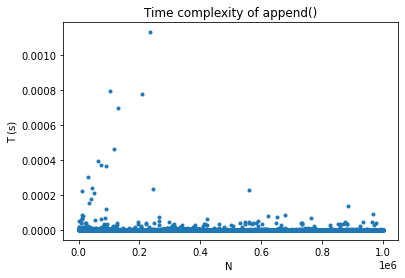
\includegraphics[width=0.6\textwidth,height=\textheight,keepaspectratio]{figure_4.png}
\caption{scatter plot for append() a single value}
\label{Figure: 4}
\end{figure}

\begin{figure}[h!]
\centering
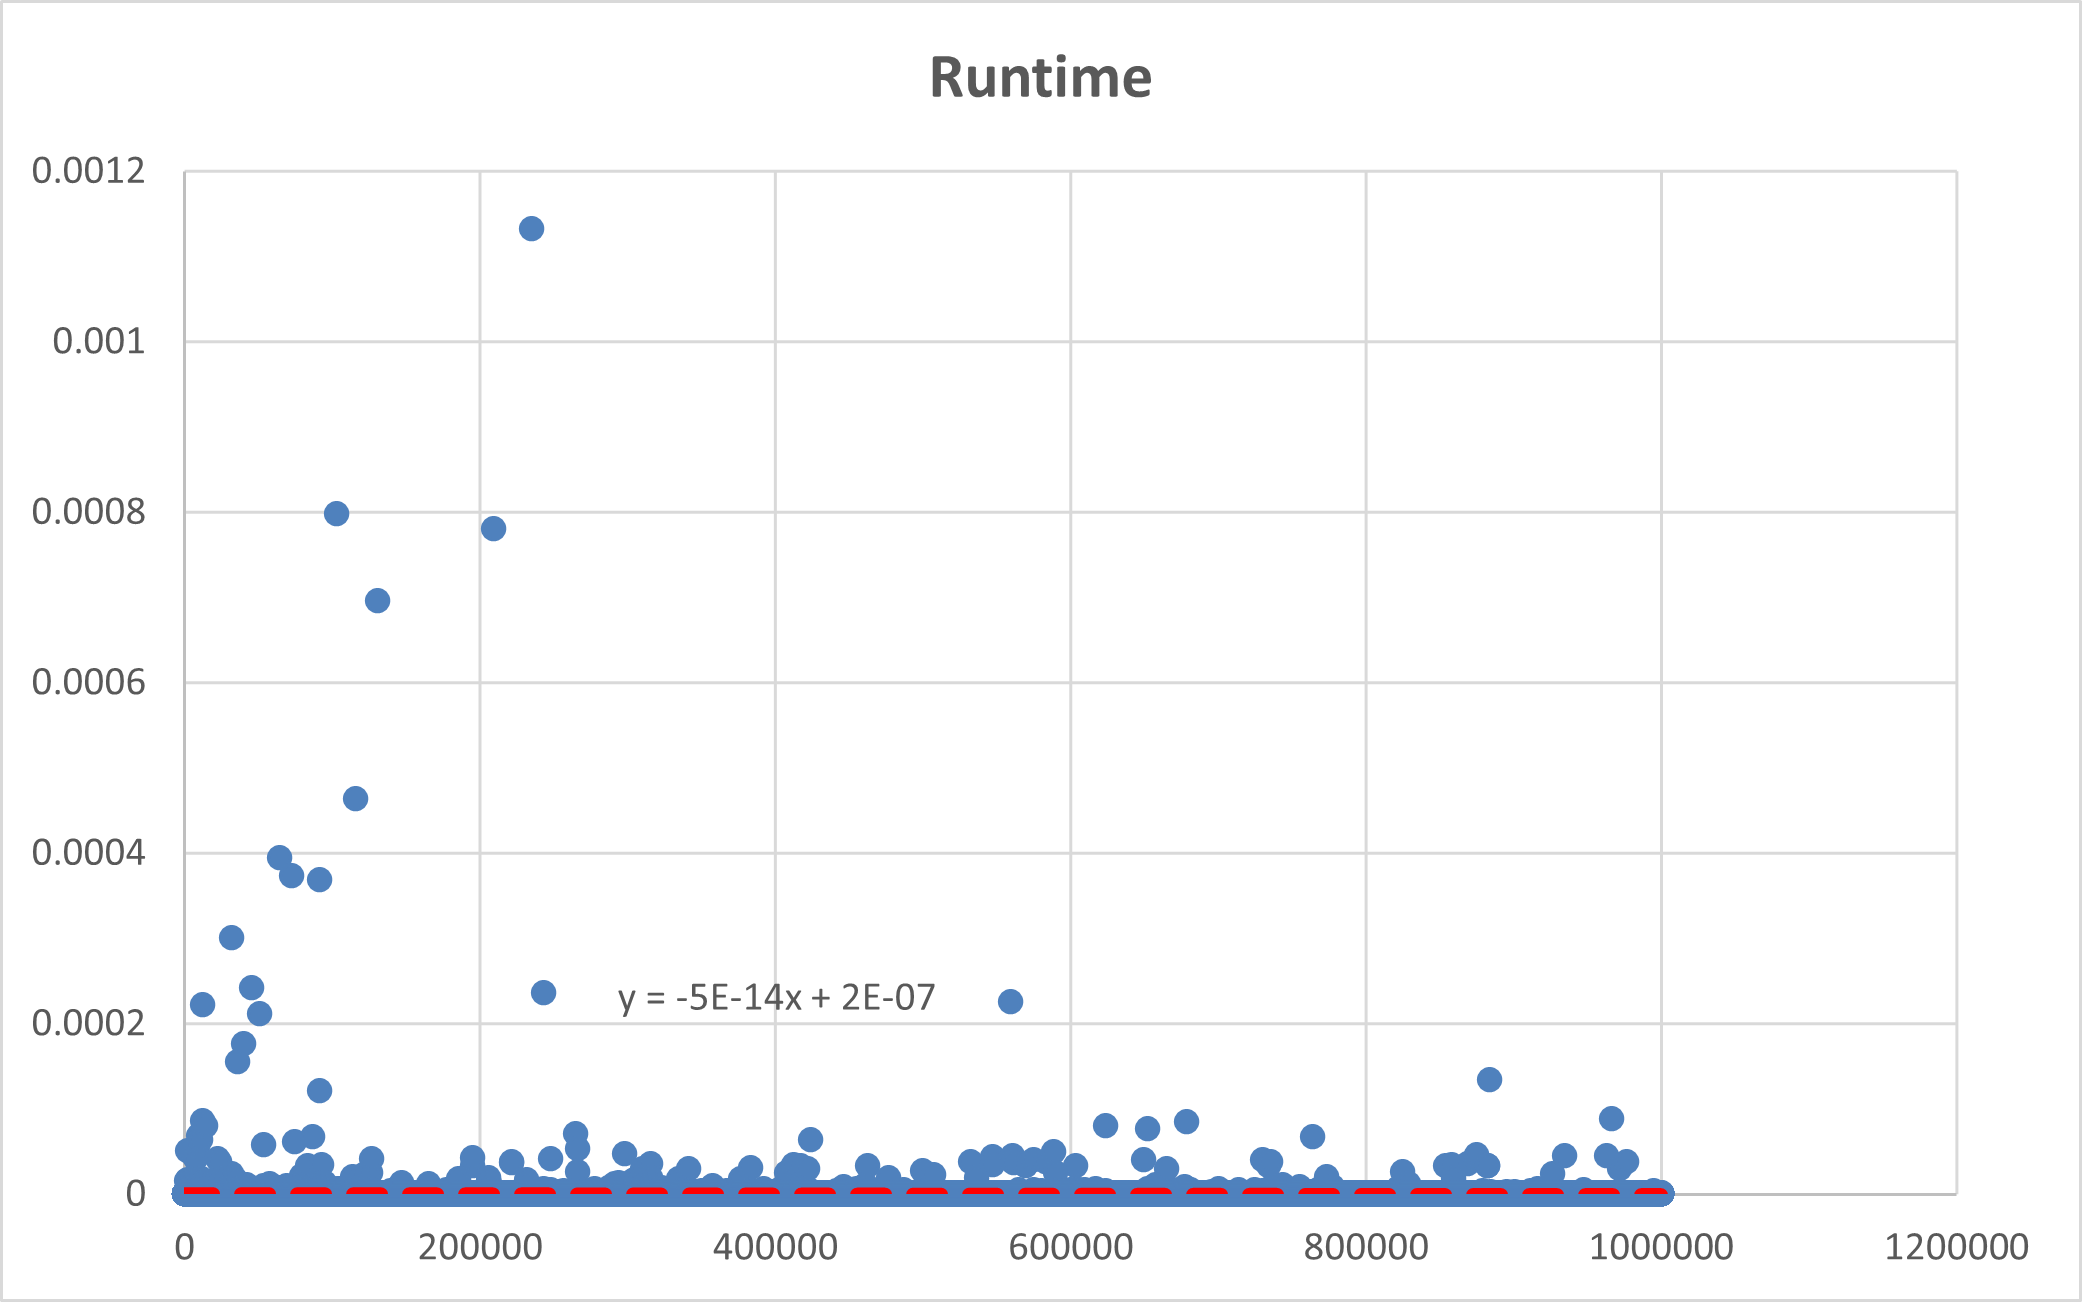
\includegraphics[width=0.6\textwidth,height=\textheight,keepaspectratio]{picture/append0.png}
\caption{constant fitting for append() a single value}
\label{append0}
\end{figure}

\newpage As showed in Figure \ref{append0}, the best fit pattern of trending line is the constant line, which demonstrates our prediction that the time complexity of \verb|append()|, i.e. \verb|list1.append(a)| is \(O(1)\). 
\item \textbf{Conclusion}\\
The time complexity of \verb|append()|, i.e. \verb|list1.append(a)| is \(O(1)\). Because this method only adds ONE elements to the end of the current list, which requires only a constant number of operations \--- no matter the size of the list. To better understand the behavior of \verb|append()|, consider this small example:
\lstset{language=Python, basicstyle=\ttfamily\small, breaklines=true, showspaces=false,
  showstringspaces=false, breakatwhitespace=true}
\begin{lstlisting}
In [1]: a = [1, 2]                                                             
In [2]: a.append([3, 4])                                                       
In [3]: a                                                                      
Out[3]: [1, 2, [3, 4]]
\end{lstlisting}
In fact, \verb|append()| really only adds one element to the end of the current list, no matter the type of the value you want to add.
\end{enumerate}

\subsection{Addition append experiment}
In this section, we want to create some additional experiments for testing the performance of \verb|append()|. In the previous test, we did the timing experiment which builds a list with one million values by appending a single value to it one step at a time.\\\\
How about appending a single list of length \verb|n| to a current list? Will the length of this appended list \verb|n| affects the running time? To answer this question, we design the following test code:
\lstset{language=Python, basicstyle=\ttfamily\small, breaklines=true, showspaces=false,
  showstringspaces=false, breakatwhitespace=true}
\begin{lstlisting}
def plot_append_ls2_test(runs):
    x = [_ * 1000 for _ in range(100)]
    y = []
    for n in x:
        for i in range(runs):
            total = 0
            ls = []
            ls2 = create_random_list(n, n)
            start = timeit.default_timer()
            ls.append(ls2)
            end = timeit.default_timer()
            total += end - start
        y.append(total/runs)
    plt.scatter(x, y, marker = '.')
    plt.xlabel('N ')
    plt.ylabel('T (s)')
    plt.title('Time complexity of append()')
    copy_test_data = workbook.add_worksheet("append_test_data2")
    copy_test_data.write(0, 0, "N")
    copy_test_data.write_column(1, 0, x)
    copy_test_data.write(0, 1, "T")
    copy_test_data.write_column(1, 1, y)
\end{lstlisting}

~\newline\noindent In this case, the output plots does not have too many outliers. So we simply set the \verb|runs|, which is the run times of the same tests for each possible value of \verb|x|, to be 1 to save the time. Each time, we add a Python list of length \verb|n| in the set of $\{0, 1000, 2000, \dots, 100000\}$ to an empty list.\\\\
Our prediction is still that the scatter diagram plotted will be a horizontal line, which means the running time of \verb|append| is irrelevant to the length of the argument list.\\\\
We do the same process as before, plot the scatter diagram and then find the best fit trending line. The result is as the following:

\begin{figure}[h!]
\centering
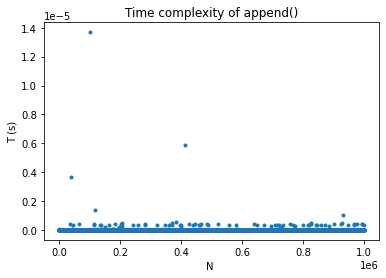
\includegraphics[width=0.6\textwidth,height=\textheight,keepaspectratio]{figure_5.png}
\caption{scatter plot for append() a list with the length $n$}
\label{Figure: 5}
\end{figure}

\begin{figure}[h!]
\centering
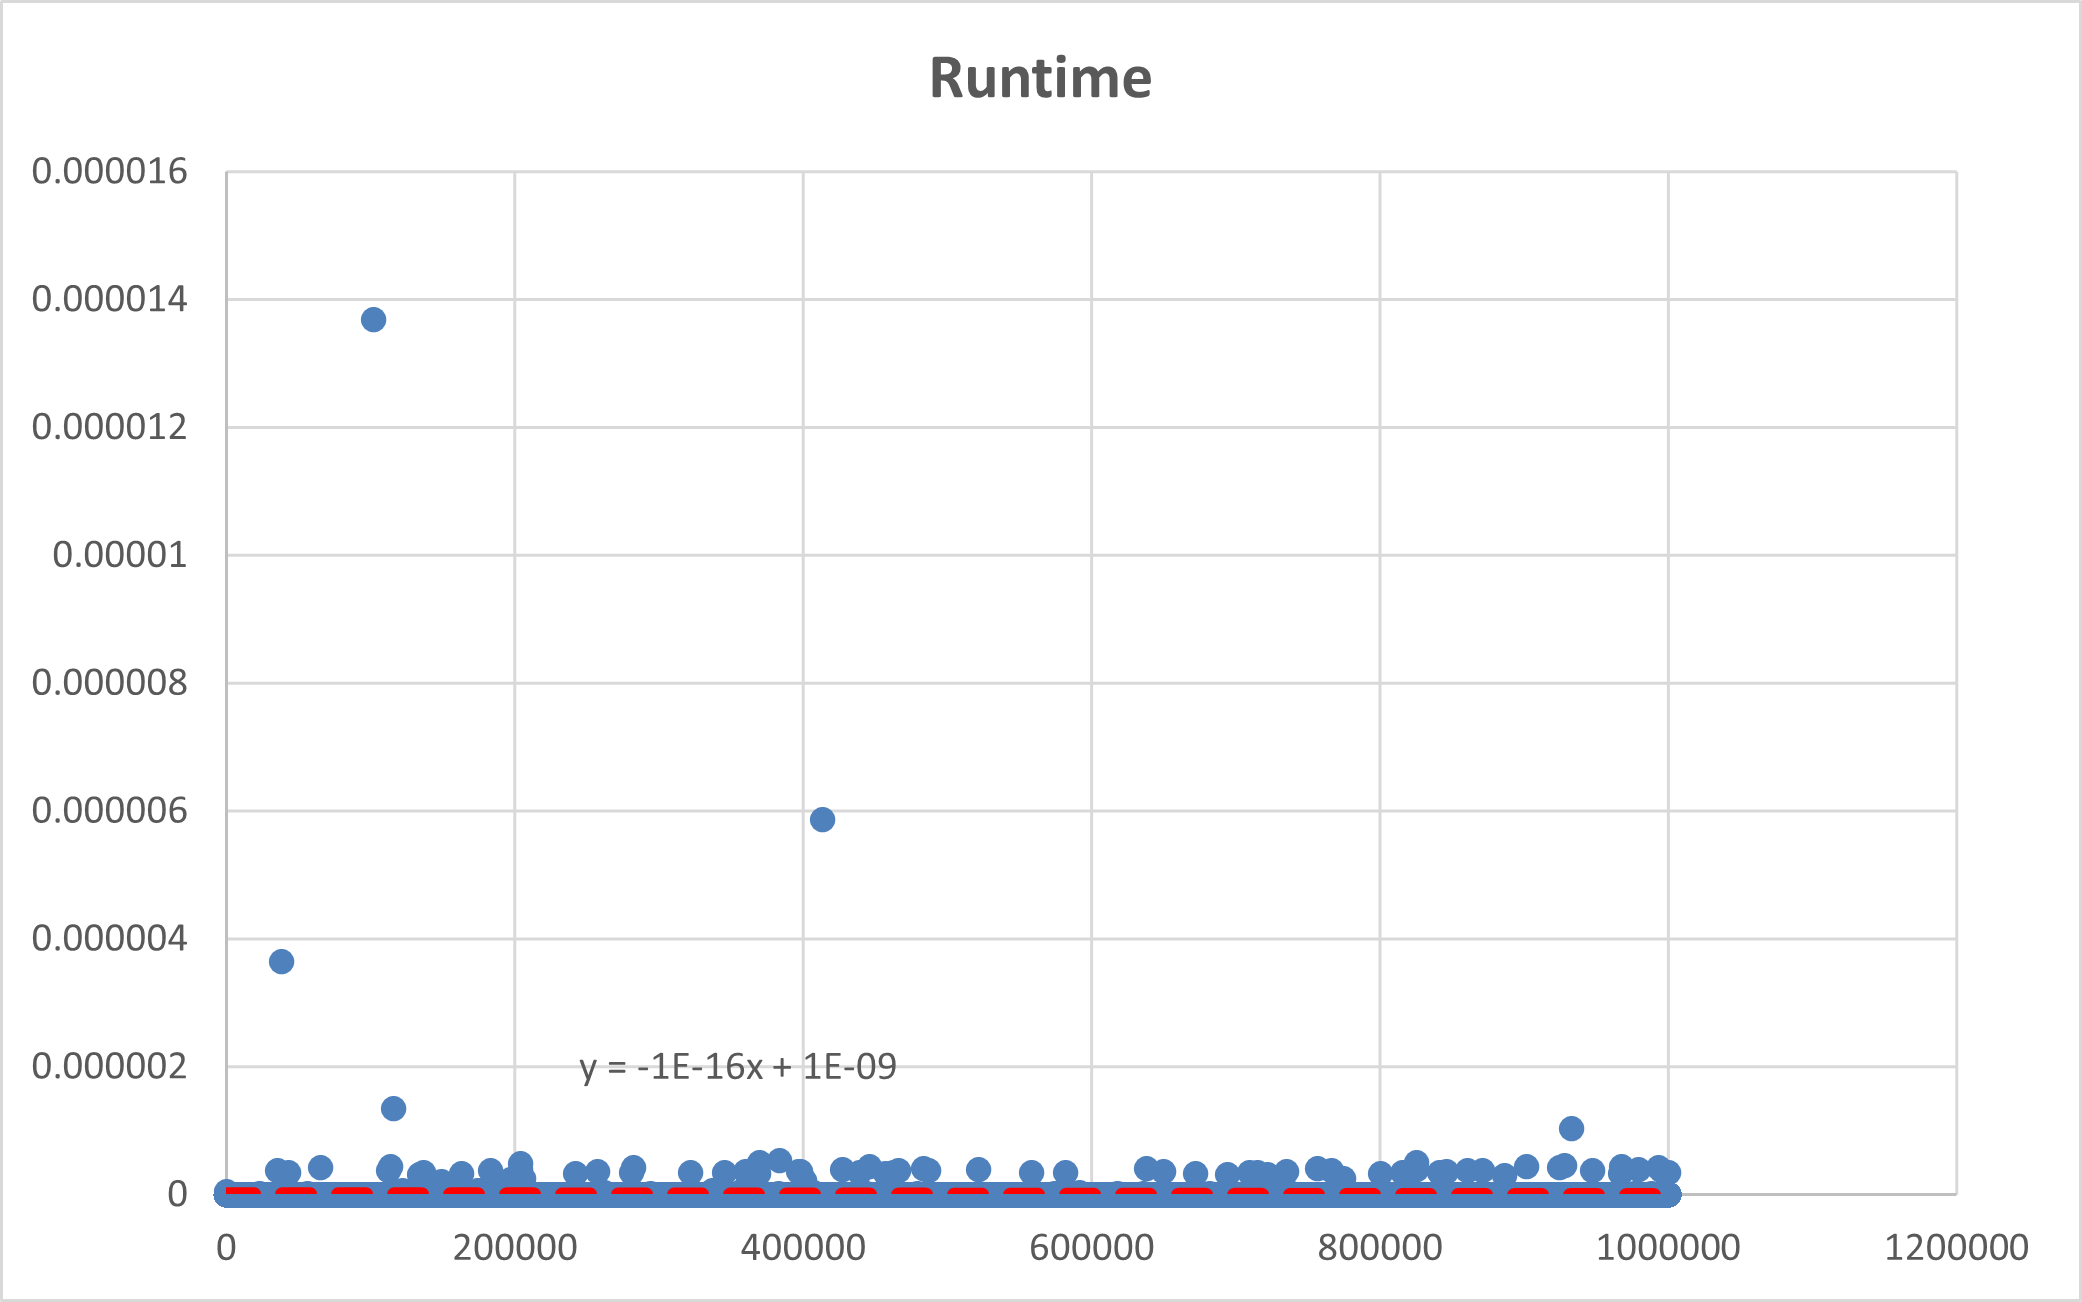
\includegraphics[width=0.6\textwidth,height=\textheight,keepaspectratio]{picture/append1.png}
\caption{constant fitting for append() a list with the length $n$}
\label{append1}
\end{figure}

\newpage ~\newline\noindent Clearly, this result verifies our prediction that the running time of \verb|append| is irrelevant to the length of the argument list.\\\\
By now, we have another question, does the length of the current object list matters, i.e. the length of \verb|a| in \verb|a.append(b)|? To answer this question, we design the following two tests:
\lstset{language=Python, basicstyle=\ttfamily\small, breaklines=true, showspaces=false,
  showstringspaces=false, breakatwhitespace=true}
\begin{lstlisting}
def plot_append_ls3_test(runs):
    x = [_ * 1000 for _ in range(100)]
    y = []
    for n in x:
        for i in range(runs):
            total = 0
            ls = create_random_list(2000, 2000)
            ls2 = create_random_list(n, n)
            start = timeit.default_timer()
            ls.append(ls2)
            end = timeit.default_timer()
            total += end - start
        y.append(total/runs)
    plt.scatter(x, y, marker = '.')
    plt.xlabel('N ')
    plt.ylabel('T (s)')
    plt.title('Time complexity of append()')
    copy_test_data = workbook.add_worksheet("append_test_data3")
    copy_test_data.write(0, 0, "N")
    copy_test_data.write_column(1, 0, x)
    copy_test_data.write(0, 1, "T")
    copy_test_data.write_column(1, 1, y)
    
def plot_append_ls4_test(runs):
    x = [_ * 1000 for _ in range(100)]
    y = []
    for n in x:
        for i in range(runs):
            total = 0
            ls = create_random_list(n, n)
            ls2 = create_random_list(n, n)
            start = timeit.default_timer()
            ls.append(ls2)
            end = timeit.default_timer()
            total += end - start
        y.append(total/runs)
    plt.scatter(x, y, marker = '.')
    plt.xlabel('N ')
    plt.ylabel('T (s)')
    plt.title('Time complexity of append()')
    copy_test_data = workbook.add_worksheet("append_test_data4")
    copy_test_data.write(0, 0, "N")
    copy_test_data.write_column(1, 0, x)
    copy_test_data.write(0, 1, "T")
    copy_test_data.write_column(1, 1, y)
\end{lstlisting}
In the first test, a list with length $n$ is appended to a list of length 2000; in the second test, a list with length $n$ is appended to a list of length $n$. Their corresponding results are showed in the following scatter diagrams.
\begin{figure}[h!]
\centering
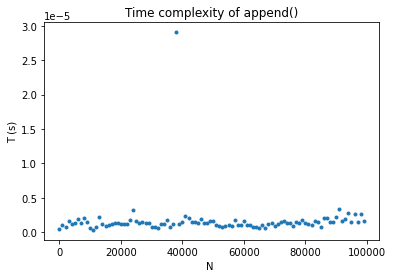
\includegraphics[width=0.5\textwidth,height=\textheight,keepaspectratio]{figure_6.png}
\caption{scatter plot for append() a $n$-length list to a $2000$-length list}
\label{Figure: 6}
\end{figure}
\begin{figure}[h!]
\centering
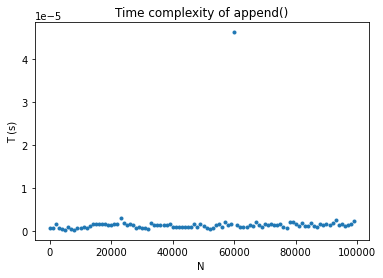
\includegraphics[width=0.5\textwidth,height=\textheight,keepaspectratio]{figure_7.png}
\caption{scatter plot for append() a $n$-length list to a $n$-length list}
\label{Figure: 7}
\end{figure}
\newpage ~\newline\noindent Apparently, both the length of the current list or the argument list does not affect the runtime of \verb|append|. This observation answer our previous questions.

\newpage

\lstset{language=Python, basicstyle=\tiny, breaklines=true, showspaces=false,
  showstringspaces=false, breakatwhitespace=true}
%\lstset{language=C,linewidth=.94\textwidth,xleftmargin=1.1cm}

\section*{Appendix: source code}
Below is all our test code for this lab, to test a single method, simply call the corresponding function, all the plot or data will be generated automatically. Note: you could need to change the path to make it work.
\noindent \lstinputlisting{source_code.py}
\end{document}

